\documentclass[handout]{beamer}
\usepackage{ctex}
\usepackage{beamerthemesplit} 
\usepackage{fontawesome}
\usepackage{graphicx}
\usepackage[framemethod=tikz]{mdframed}
\usepackage{tikz}
\usepackage{epstopdf}
\usetikzlibrary{arrows,decorations.markings}
\usetikzlibrary{decorations.pathreplacing}
\usetikzlibrary{calc}
\usetheme{Boadilla}

\newmdenv[tikzsetting={draw=black,fill=white,fill opacity=0.7, line width=3pt},
backgroundcolor=none,leftmargin=0,rightmargin=40,innertopmargin=3pt]
{titleBox}
	\title[课堂测验题解]{2016/4/5计算机网络课堂测试讲解}
	\author[\faEnvelope{} \href{mailto:cippusmcm@163.com}{\textit{i@xyli.me}}]{Xinyi Li}
\institute[]{\faChain{} \url{https://www.yangzhou301.com/2016/04/07/471457613/}}
\date{\today}

\begin{document}
	\linespread{1}
	{
		\usebackgroundtemplate{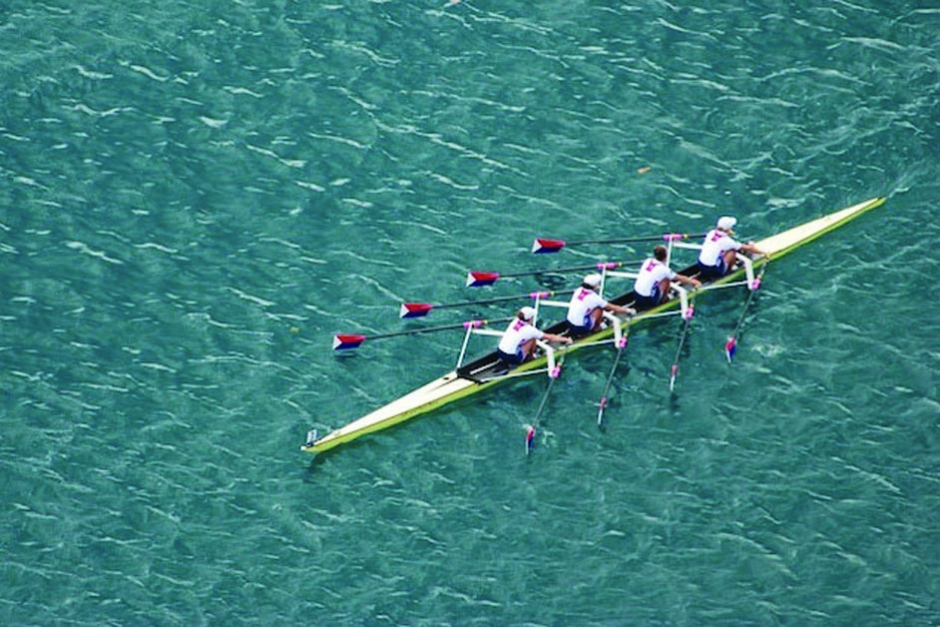
\includegraphics[height=\paperheight]{exciting.jpg}}
		\begin{frame}[plain]
			\vspace{13em}
			\begin{titleBox}
				{\centering{\LARGE \inserttitle}
				}\\
				\insertinstitute \\ \faCalendarCheckO{ }\insertdate
			\end{titleBox}
		\end{frame}
	}
	\section{课序号02}
	\subsection{1.TCP连接}
	\begin{frame}{第一题}
		客户端A和服务器端B进行了TCP通信。初始序列号都为0。连接建立后,A以500B的传输单元向B传输5kB的数据。其中第二个数据单元丢失,并重传了2次;B向A发送10kB的数据(传输单元也为500B),数据和ACK都没有丢失。所有的数据传输完毕后,TCP连接关闭(其中A先发起关闭)。
		\begin{enumerate}
			\item 画出TCP连接建立的过程(连接建立过程中没有丢包);
			\item 	画出关闭TCP连接的完整过程。
		\end{enumerate}
		要求标出必要的标识位、序列号、确认号等。
	\end{frame}
	
	\begin{frame}{建立连接}
	\framesubtitle{三次握手}
	\begin{enumerate}
		\item 客户端A给服务器B发送一个SYN请求给服务器B要求建立连接,生成一个随机数作为初始序列号seq=X,
		\item 服务器B收到请求,回应SYN-ACK表示服务器B能接收到客户端的数据且允许建立连接,其中ack=X+1,这个确认号表示接收到了序列号为X的分片,请求发送下一个分片。而这个SYN-ACK消息本身的序列号由B随机生成seq=Y
		\item 客户端A收到SYN-ACK,回应一个ACK给服务器B表示客户端能接收到服务器的数且允许建立连接,seq=X+1(也就是B发送的ack),并表示接下来希望接收的服务器发来的数据为ack=Y+1
	\end{enumerate}
	\end{frame}
	
	\begin{frame}{建立连接}
		\framesubtitle<1>{A和B的初始序列号为0,A向B发送SYN请求建立连接}
		\framesubtitle<2>{B回应SYN-ACK允许请求}
		\framesubtitle<3>{A回应ACK表示客户端能接收到服务器的数且允许建立连接}
		\begin{center}
\begin{tikzpicture}[decoration={
	markings,
	mark=at position 1 with {\arrow[scale=1]{angle 90}};
},scale=0.8]
  \draw[->,dashed,line width=2,color=gray] (0,-0.5) node[above,color=black]{\large{$A$}} -- (0,-9);
  \draw[->,dashed,line width=2,color=gray] (8,-0.5) node[above,color=black]{\large{$B$}} -- (8,-9);
  \draw<1->[->,line width=1,postaction={decorate}] (0,-1) --node[above,sloped]{\texttt{SYN=1, seq=0}} (8,-3);
  \draw<2->[->,line width=1,postaction={decorate}] (8,-3.1) --node[above,sloped]{\texttt{SYN=1, seq=0, ack=1}} (0,-5.1);
  \draw<3->[->,line width=1,postaction={decorate}] (0,-5.2) --node[above,sloped]{\texttt{{\textcolor{gray}{SYN=0, }
  		}seq=1, ack=1}} (8,-7.2);
\end{tikzpicture}
\end{center}
\end{frame}

\begin{frame}{数据传输}
	\framesubtitle{A发送给B的第一个数据单元}
	\begin{center}
		\begin{tikzpicture}[decoration={
			markings,
			mark=at position 1 with {\arrow[scale=1]{angle 90}};
		},scale=0.7]
		
  \draw[->,dashed,line width=2,color=gray] (0,-0.5) node[above,color=black]{\large{$A$}} -- (0,-9);
  \draw[->,dashed,line width=2,color=gray] (8,-0.5) node[above,color=black]{\large{$B$}} -- (8,-9);
  \draw[->,line width=1,postaction={decorate}] (0,-1) --node[above,sloped]{\texttt{SYN=1, seq=0}} (8,-3);
  \draw[->,line width=1,postaction={decorate}] (8,-3.1) --node[above,sloped]{\texttt{SYN=1, seq=0, ack=1}} (0,-5.1);
  \draw[->,line width=1,postaction={decorate}] (0,-5.2) --node[above,sloped]{\texttt{seq=1, ack=1}} (8,-7.2);
%  \draw[->,line width=1,postaction={decorate}] (0,-7.5) --node[above,sloped]{\texttt{seq=2, 500B数据}} (8,-9.5);
%  \draw[->,line width=1,postaction={decorate}] (8,-9.7) --node[above,sloped]{\texttt{ACK=1, ack=502}} (0,-11.7);

	    \draw [decorate,decoration={brace,amplitude=10pt,mirror}]
		(-0.1,-1) --node [black,midway,below,sloped,yshift=-10pt] {建立连接}  (-0.1,-7.2);
		\draw [decorate,decoration={brace,amplitude=10pt,mirror},color=blue]
		(-0.1,-7.5) --node [black,midway,below,sloped,yshift=-10pt,xshift=-1cm,color=blue] {发送数据}  (-0.1,-12);
		
		\end{tikzpicture}
	\end{center}
	
\end{frame}

\begin{frame}{数据传输}
	\framesubtitle{接下来可能的情况}
	\begin{block}{}
		连接建立后,A以\textcolor<2->{gray}{500B}的传输单元向B传输\textcolor<2->{red}{5kB}的数据。其中\textcolor<2->{gray}{第二个数据单元丢失,并重传了2次};B向A发送\textcolor<2->{red}{10kB}的数据(传输单元也为\textcolor<2->{gray}{500B}),\textcolor<2->{gray}{数据和ACK都没有丢失}。
	\end{block}
	\begin{itemize}[<2->]
		\item 停止等待(\textit{Stop-and-wait})
		\item 退回N步(\textit{Go Back N})
		\item 选择重传(\textit{Selective Repeat})
	\end{itemize}
	\begin{alertblock}<3>{但这些都不会影响seq和ack最后的编号}
		\begin{itemize}
			\item 可靠数据传输:收到的分片必须有序,重传的分片序列号seq必然与原分片相同
			\item 只有当上一个分片传输了数据(包括SYN和FIN也算在内),且不是重传的情况下,下一个分片的seq才可以增加
		\end{itemize}
	\end{alertblock}
\end{frame}

\begin{frame}{数据传输}
	\framesubtitle{一种可能的情况(选择重传)}
	\begin{center}
	\begin{tikzpicture}[decoration={
		markings,
		mark=at position 1 with {\arrow[scale=1]{angle 90}};
	},scale=.43]
	
  \draw[->,dashed,line width=2,color=gray] (0,-0.5) node[above,color=black]{\large{$A$}} -- (0,-17.5);
  \draw[->,dashed,line width=2,color=gray] (8,-0.5) node[above,color=black]{\large{$B$}} -- (8,-17.5);
  \draw[->,line width=1,color=blue,postaction={decorate}] (0,-1) --node[above,sloped,pos=0.25]{\texttt{seq=1, 500B数据}} (8,-3);
  \draw[->,line width=1,postaction={decorate}] (8,-3.1) --node[above,sloped,pos=0.25]{\texttt{ack=501,\textcolor{gray}{seq=1}}} (0,-5.1);
  \draw[->,line width=1,color=red,postaction={decorate}] (0,-2) --node[above,sloped,pos=0.333]{\texttt{seq=501, 500B数据}} (6,-3.5) node[right]{\large{\faClose}};
  \draw[->,line width=1,color=blue,postaction={decorate}] (0,-3) --node[above,sloped,pos=0.25]{\texttt{seq=1001, 500B数据}} (8,-5);
  \draw[->,line width=1,color=blue,postaction={decorate}] (0,-4) --node[above,sloped,pos=0.25]{\texttt{seq=1501, 500B数据}} (8,-6);
  \draw[->,line width=1,postaction={decorate}] (8,-5.1) --node[above,sloped,pos=0.25]{\texttt{ack=1501,\textcolor{gray}{seq=1}}} (0,-7.1);
  \draw[->,line width=1,postaction={decorate}] (8,-6.1) --node[above,sloped,pos=0.25]{\texttt{ack=2001,\textcolor{gray}{seq=1}}} (0,-8.1);
  \draw[->,line width=1,color=red,postaction={decorate}] (0,-8.5) --node[above,sloped,pos=0.333]{\texttt{seq=501, 500B数据}} (6,-10) node[right]{\large{\faClose}};
  \draw[->,line width=1,color=blue,postaction={decorate}] (0,-10.5) --node[above,sloped,pos=0.25]{\texttt{seq=501, 500B数据}} (8,-12.5);
  \draw[->,line width=1,postaction={decorate}] (8,-12.6) --node[above,sloped,pos=0.25]{\texttt{ack=1001,\textcolor{gray}{seq=1}}} (0,-14.6);
  \draw[->,line width=1,color=blue,postaction={decorate}] (0,-14.8) --node[above,sloped,pos=0.25]{\texttt{seq=2001, 500B数据}} (8,-16.8);
  \draw (4, -16.5) node {$\vdots$}

	\end{tikzpicture}
	\end{center}
\end{frame}

\begin{frame}{关闭连接}
	\framesubtitle{四次挥手}
	\begin{enumerate}
		\item 客户端A向服务器B发送一个FIN请求关闭连接
		\item 服务器B接收到请求后回应一个ACK表示允许关闭连接,至此A$to$B的连接已经关闭,A不能再向B发送数据,这是半关闭(\textit{half-closed})状态
		\item 服务器B向客户端A发送一个FIN请求关闭连接
		\item 客户端A接收到请求后回应一个ACK表示允许关闭连接,至此连接关闭
	\end{enumerate}
	\begin{block}<2>{}
		数据传输结束后的初始序列号和确认号:
		\begin{itemize}
			\item A: $seq=5001$,$ack=10001$
			\item B: $seq=10001$,$ack=5001$
		\end{itemize}
	\end{block}
\end{frame}

\begin{frame}{关闭连接}
	\framesubtitle<1>{客户端A向服务器B发送一个FIN请求关闭连接}
	\framesubtitle<2>{服务器B接收到请求后回应一个ACK表示允许关闭连接}
	\framesubtitle<3>{服务器B向客户端A发送一个FIN请求关闭连接}
	\framesubtitle<4>{客户端A接收到请求后回应一个ACK表示允许关闭连接}
	\begin{center}
		\begin{tikzpicture}[decoration={
			markings,
			mark=at position 1 with {\arrow[scale=1]{angle 90}};
		},scale=0.7]
		\draw[->,dashed,line width=2,color=gray] (0,-0.5) node[above,color=black]{\large{$A$}} -- (0,-10);
\draw[->,dashed,line width=2,color=gray] (8,-0.5) node[above,color=black]{\large{$B$}} -- (8,-10);
\draw<1->[->,line width=1,postaction={decorate}] (0,-1) --node[above,sloped]{\texttt{FIN=1, seq=5001}} (8,-3);
\draw<2->[->,line width=1,postaction={decorate}] (8,-3.1) --node[above,sloped]{\texttt{ACK=1, seq=10001, ack=5002}} (0,-5.1);
\draw<3->[->,line width=1,postaction={decorate}] (8,-5.2) --node[above,sloped]{\texttt{FIN=1, seq=10001}} (0,-7.2);
\draw<4->[->,line width=1,postaction={decorate}] (0,-7.3) --node[above,sloped]{\texttt{ACK=1, seq=5002, ack=10002}} (8,-9.3);

		\end{tikzpicture}
	\end{center}
\end{frame}

\subsection{2.路由选择}
\begin{frame}{第二题}
	某路由器路由表如下表所示,现在收到5个分组,其目的IP地址分别为:
	\begin{table}
		\begin{tabular}{|c|c|c|}
			\hline
			目的IP地址&子网掩码&下一跳路由器 \\
			\hline
			128.96.39.0&255.255.255.128&接口$0$ \\
			\hline
			128.96.39.128&255.255.255.128&接口$1$\\
			\hline
			128.96.40.0&255.255.255.128&$R_2$\\
			\hline
			192.4.153.0&255.255.255.192&$R_3$\\
			\hline
			默认& &$R_4$\\
			\hline
		\end{tabular}
	\end{table}
	分别计算并写出下一跳路由器
	\begin{enumerate}
		\item 128.96.39.10
		\item 128.96.40.12
		\item 128.96.40.151
		\item 192.4.153.17
		\item 192.4.153.90
	\end{enumerate}
\end{frame}

\begin{frame}
	\begin{block}{}
	将IP地址和子网掩码作\textcolor{blue}{与运算},找到目的IP地址和运算结果一致的路由项,若不存在,则走\textcolor{blue}{缺省路由}
	\end{block}
	\begin{description}
		\item<2->[128.96.39.10] 和255.255.255.128相与得到	128.96.39.0,下一跳为接口$0$
		\item<3->[128.96.40.12] 和255.255.255.128相与得到128.96.40.0,下一跳$R_2$
		\item<4->[128.96.40.151]和255.255.255.128相与得到128.96.40.128不在目的IP地址表中,再与255.255.255.192的运算结果为128.96.40.128不在目的IP地址表中,所以走缺省路由$R_4$
		\item<5->[192.4.153.17]和255.255.255.128相与得到192.4.153.0不在目的IP地址表中,与255.255.255.192的运算结果为192.4.153.0,下一跳$R_3$
		\item<6->[192.4.153.90]和255.255.255.128相与得到192.4.153.0不在目的IP地址表中,与255.255.255.192的运算结果为192.4.153.64不在目的IP地址表中,所以走缺省路由$R_4$
	\end{description}
\end{frame}

\section{课序号01}
\subsection{1.TCP报文结构}
\begin{frame}{第一题}
	一个TCP的首部字节数据见下表所示,回答下列问题:
	\begin{table}
		\begin{tabular}{|c|c|c|c|c|c|c|c|c|c|}
			\hline
			编号&	1& 	2&	3&	4&	5& 6&	7&	8&	9\\
			\hline
			数据&	0d&	28&	00&	15&	00&	5f&	a9&	06&	00\\
			\hline
			编号&	10&	11&	12&	13&	14&	15&	16&	17&	18\\
			\hline
			数据&	00&	00&	00&	70&	02&	40&	00&	C0&	29\\
			\hline
			编号&	19&	20& & & & & & & \\ 	
			\hline						
			数据&	00&	00&	& & & & & & \\	
			\hline						
		\end{tabular}
	\end{table}
	\begin{enumerate}
		\item 源端口号是多少?目的端口号是多少?
		\item 发送的序列号是多少?确认号是多少?
		\item TCP首部的长度是多少?
		\item 这是一个使用什么协议的TCP连接?(\textcolor{red}{提示}:观察端口号)该TCP连接的状态是什么?	
	\end{enumerate}
\end{frame}

\begin{frame}{TCP报文结构}
	\begin{figure}
			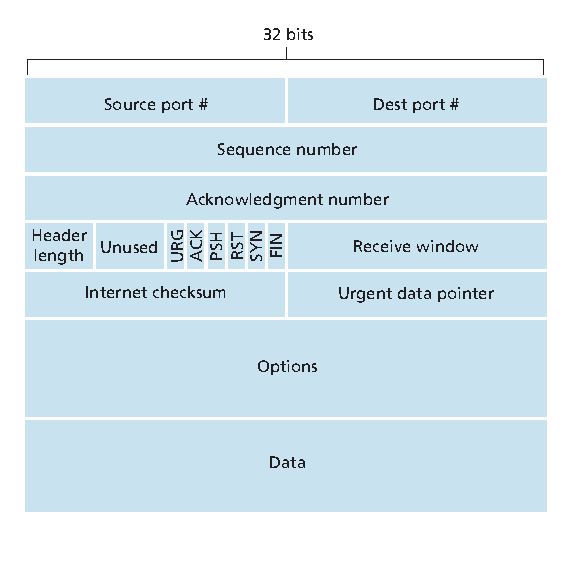
\includegraphics[scale=.8]{seg.pdf}
	\end{figure}
	
\end{frame}

\begin{frame}{寻找对应字段}
	\framesubtitle{注意这里编号从1开始}
	\begin{description}
		\item<2->[源端口号] 编号1-2的数据为0d28,转换为十进制数3368
		\item<3->[目的端口号] 编号3-4的数据为0015,转换为十进制数21,\textcolor{blue}{这是一个FTP连接}
		\item<4->[序列号] 编号5-8的数据为005fa906,转换为十进制数6269190
		\item<5->[确认号] 编号9-12的数据为00000000,转换为十进制数0
		\item<6->[首部长度] 编号13的前4位,对应的数值为7
		首部长度字段的单位是字(4B,32bit),也就是说这个报文的首部长度是28B
		\end{description}
\end{frame}

\begin{frame}{TCP连接状态}
	\framesubtitle{注意SYN、ACK、FIN标识位}
	\begin{description}
		\item[ACK] 编号14的第4位,数值为0,该消息没有捎带ACK
		\item[SYN] 编号14的第7位,数值为1,发送了一个SYN消息
		\item[FIN]编号14的第8位,数值为0,没有捎带FIN
	\end{description}
	{ack确认号为0,说明没有收到对方发来的数据(同步未进行),因此这是一个发起的SYN请求,是TCP建立连接时三次握手的第一条消息,这个连接在建立状态。}
	\begin{center}
		\begin{tikzpicture}[decoration={
			markings,
			mark=at position 1 with {\arrow[scale=1]{angle 90}};
		},scale=0.4]
		{\scriptsize 
		\draw[->,dashed,line width=2,color=gray] (0,-0.5) node[above,color=black]{\large{$A$}} -- (0,-9);
		\draw[->,dashed,line width=2,color=gray] (8,-0.5) node[above,color=black]{\large{$B$}} -- (8,-9);
		\draw[->,color=red,line width=1,postaction={decorate}] (0,-1) --node[above,sloped]{\texttt{SYN=1, seq=0}} (8,-3);
		\draw[->,line width=1,postaction={decorate}] (8,-3.1) --node[above,sloped]{\texttt{SYN=1, seq=0, ack=1}} (0,-5.1);
		\draw[->,line width=1,postaction={decorate}] (0,-5.2) --node[above,sloped]{\texttt{{\textcolor{gray}{SYN=0, }
				}seq=1, ack=1}} (8,-7.2);}
		\end{tikzpicture}
	\end{center}
\end{frame}

\subsection{2.地址分配}
\begin{frame}{第二题}
	一个自治系统有5个局域网,如下图所示。LAN2至LAN5上的主机数分别是91、150、3和15,该自治系统分配到的IP地址块为30.138.118/23,试给出每个局域网的地址块。(\textcolor{red}{提示}:路由器(包括边界路由器)也需占用一个IP地址)
	\begin{center}
	\begin{tikzpicture}[scale=0.5]
	
	{\scriptsize 
\draw[-,thick] (-4,0) -- node[below,label=below:LAN1]{
\includegraphics[scale=.7]{icon/webcluster}} (8,0) ;
\draw[-,thick] (-3,0) -- node[label=left:\textbf {路由器}]{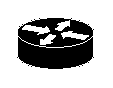
\includegraphics[scale=.7]{icon/router}} (-3,4) node[above,yshift=-5pt,label=above:LAN2: \textbf {91台主机}]{
\includegraphics[scale=.7]{icon/webcluster}};
\draw[-,thick] (2,0) -- node[label=left:\textbf {路由器}]{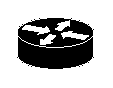
\includegraphics[scale=.7]{icon/router}} (2,4) node[above,yshift=-5pt,label=above:LAN3: \textbf {150台主机}]{
\includegraphics[scale=.7]{icon/webcluster}};
\draw[-,thick] (7,0) -- node[label=left:\textbf {路由器}]{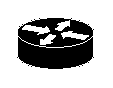
\includegraphics[scale=.7]{icon/router}} (7,4) node[above,yshift=-5pt,label=above:LAN4: \textbf {3台主机}]{
\includegraphics[scale=.7]{icon/webcluster}};
\draw[-,thick] (7,2) -- (10,2) node[right,xshift=-5pt,label=above:LAN5: \textbf {15台主机}]{
\includegraphics[scale=.7]{icon/webcluster}};
}
	\end{tikzpicture}
	\end{center}
\end{frame}

\begin{frame}{分配原则}
	\begin{itemize}
		\item 有多种分配方案
		\item 优先考虑主机数多的局域网
		\item 主机数$x$,连接的路由数$y$,那么分配的主机地址数$n$需要满足
		$$2^{n-1} \le x+y < 2^n$$
	\end{itemize}
\end{frame}

\begin{frame}{一种可行的分配方案}
	\framesubtitle{仅供参考}
	\begin{description}
		\item[LAN3]有150台主机和一个路由器,需要8位的主机地址。网络地址则是剩下的24位,取IP地址的第24位为0,将30.138.118.0/24分配给LAN3
		\item[LAN2]有91台主机和一个路由器,需要7位的主机地址。网络地址则是剩下的25位,可以取IP地址的第24位为1,第25位为0,将30.138.119.0/25分配给LAN2
		\item[LAN5]有15台主机和一个路由器,需要5位主机地址,剩下27位为网络地址,取24,25,26,27位为1110,将30.138.118.192/27分配给LAN5
	\end{description}
\end{frame}

\begin{frame}{一种可行的分配方案}
	\framesubtitle{仅供参考}
	\begin{description}
	\item[LAN1]有三个路由,而且作为自治域至少要有一个边界路由与其他自治域相连,所有至少需要4个IP,取3位作为主机地址,IP地址的第24,25,26,27,28,29位可以取111101,分配地址段30.138.119.232/29
	\item[LAN4] 有3台主机和一个路由同理使用3位主机地址,第24,25,26,27,28,29位可以取111110,分配地址段30.138.119.240/29
	\end{description}
\end{frame}

\subsection{3.零压缩}
\begin{frame}{第三题*}
	将以下IPV6地址用零压缩方法写成简洁形式。
	\begin{enumerate}
		\item 0000:0000:0F53:6382:AB00:67DB:BB27:7332
		\item 0000:0000:0000:0000:0000:0000:004D:ABCD
		\item 0000:0000:0000:AF36:7328:000A:87AA:0398
		\item 2819:00AF:0000:0000:0000:0035:0CB2:B271
	\end{enumerate}
	
\end{frame}

\begin{frame}{前导零压缩}
	\begin{itemize}
		\item 如果一个位段为0000,那么可以用0进行代替。
		\item IPv6每段地址前端的0可以省略,中间和后端则不可以。
		\item 几个连续的位段为0,可以用::代替这些0。
	    \item ::在IPv6中只能出现一次。
	\end{itemize}
\end{frame}

\begin{frame}{答案}
\begin{itemize}
	\item ::F53:6382:AB00:67DB:BB27:7332
	\item ::4D:ABCD
	\item ::AF36:7328:A:87AA:398
	\item 2819:AF::35:CB2:B271
\end{itemize}	
\end{frame}

\end{document}